\begin{abstract}
A multifidelity approach for the solution of aeroelastic optimization problems is developed using open-source tools. The Multidisciplinary Optimization problem is managed via OpenMDAO and a dedicated python library. High fidelity aerodynamics are handled with ADFlow, whilst PANAIR solves the low fidelity calls. Structural displacements are computed via NASTRAN95 and transferred to the aerodynamic mesh with radial basis functions. The program starts optimizing the problem at a low fidelity level, and once some predefined constraint convergence tolerance is reached, the high fidelity solver is called.  The final goal of this project is to apply the methodology to the optimization of a Blended Wing Body (BWB) concept aircraft. 

\end{abstract}

\keywords{Multifidelity, aeroelasticity, BWB, MDO}
\printnomenclature


\section{Introduction}
\label{sec:introduction}

Modern engineering design problems rely increasingly on the interdisciplinary interactions between subsystems. As a consequence, multidisciplinary design strategies have been developed, these allow to manipulate design variables from various disciplines simultaneously. Moreover, the incorporation of optimization tools within these methodologies leads to what is referred collectively as Multidisciplinary Design Optimization (MDO).    
The present work deals with the interaction of aerodynamics and structures (so called Fluid-Structure Interaction, FSI), which is a key feature in aircraft design. Coupled aeroelastic analyses allow a better prediction of the aerodynamic forces and structural displacements that the aircraft experiences in real flight, hence, an MDO platform is implemented in order to study these interactions. \par 
Each discipline inside the MDO problem requires a solver that computes its effects on the global problem, with the aerodynamic solution being the main source of computational cost. High fidelity CFD analyses offer accurate results, but at the expense of high computational time. On the other hand, potential flow theory, and its computational implementation, the panel codes, offer reasonable approximations with low computational demands. The main goal of this project is to efficiently use low-fidelity analyses, combined to high-fidelity ones, to conduct aeroelastic optimizations, with an application to a Blended Wing Body (BWB) configuration.  
\section{Semester 2 section}
\label{sec:projectissues}
The development of a multifidelity method for aeroelastic analysis requires a coordinated implementation for the high-fidelity and low-fidelity models. In order to achieve this, a management strategy must be implemented. Commonly used alternatives include: Trust Region Model Management (TRMM), Bayesian Regression, Co-kriging \cite{peherstorfer2018survey}. A detailed review of these strategies is given in subsec. \ref{subsec:sota}. Another important part of this step is to define the criteria that triggers the alternation between fidelities.

Once a management strategy has been chosen, the next step is to implement said model in the OpenMDAO platform. The resulting code has to be applicable to general cases and not just the particular one discussed in this work. Finally, the multifidelity method will be used for the aeroelastic optimization of a Blended Wing Body. The main issue at this point is the validation of the results because there are few well documented cases of BWB concepts \cite{Quinlan2019, Bryson2019} that can be used as reference for the present work. 

\subsection{Context and key issues}
Coupled FSI simulations are the most accurate way to represent aeroelastic phenomena. However, their computational cost  remains too expensive for engineering design and optimization. Low-fidelity models are used instead, such as the linearized potential flow approximation. These models are considerably cheaper than RANS solvers and perform well in the low subsonic regime \cite{Marques2019}. Nevertheless, there are important non-linear phenomena that are not adequately represented by linearized potential flow models. For this reason, there is a great interest in developing strategies that ease the computing load of the solution while preserving the accuracy of the final solutions. \par
The present method leverages information from low-fidelity aeroelastic models to optimize a BWB (or any other aerodynamic structure) at a reasonable cost. The multifidelity method has three main parts: 
\begin{itemize}
    \item A multidisciplinary platform that couples the aerodynamic effects to the structural displacements.
    \item A set of solvers for aerodynamic and structural problems.
    \item A management strategy that assigns the high or low fidelity software according to given criteria.
\end{itemize}\par
At the beginning of this period, the main task was to define the scope of the problem, the objectives and the schedule for the core activities. Next, a state of the art review was needed so that the current strategies and methodologies carried out by the researchers of the field around the world could be taken into account for the present work. Then, as this project relies heavily on the use of open-source tools and python libraries developed previously, a key issue was to get the whole set of programs working together properly. The task took significantly longer than expected due to compatibility problems between recently released versions and cross-platform consistency. Once this was solved, the project started to advance faster. It is expected that over the course of the next period, there will be enough time to overcome the delays of the present one. 

\subsection{State of the art}
\label{subsec:sota}
The starting point for the bibliography research is a Survey of Multifidelity Methods by Peherstorfer \cite{peherstorfer2018survey}, where a variety of alternatives are listed and classified. Surrogate modelling is a global optimization strategy. It uses co-kriging (see subsec. \ref{subsubsec:kriging} for details) as a regression technique in order to link High-Fidelity sources with one or many Low-Fidelity functions. This correlated model can be used to find optimal solutions faster \cite{Forrester2007}. On the other hand, simpler approaches such as a linear regression are found to offer a good balance between accuracy, cost and simplicity \cite{Zhang2019}. Other advantages include: ease to combine many low-fidelity sources and robustness for High-Fidelity samples with the presence of noise \cite{Zhang2019}. 

Newton methods and their variations have been explored as well. Jovanov and Breuker propose to solve the High-Fidelity problem by adding an aerodynamic correction load to the solution of the Low-Fidelity equation. The defect-correction method accelerates the convergence compared to the Quasi-Newton method \cite{Jovanov2015}. This last case does not consider the methods as black-boxes, but rather exploits the fact that the algorithms of both fidelity levels are known and can be modified at any stage to accommodate the necessary corrections between them. Scholz presents an Aggressive Space Mapping methodology, it solves for the low fidelity fluid–structure interaction solution and then feeds that information to a Quasi-Newton algorithm. The final results are obtained from a mapping function between both fidelity levels \cite{Scholcz2014}. 

When it comes to the application of mutifidelity models to aerospace design, there are several publications on the subject. A Bayesian-enhanced Low-Fidelity correction proved the ability to maintain high-fidelity accuracy while reducing computational cost associated with the optimization of an airfoil shape \cite{fischer2018bayesian}. An aeroelastic optimization of a BWB was carried out by Bryson \cite{Bryson2019} using a new TRMM (Trust Region Model Management) approach (see subsec. \ref{subsubsec:TRMM}). Its main difference is that it adds hybrid additive-multiplicative corrections (or bridge functions) to the low-fidelity analysis \cite{Bryson2019a}. Another approach to the aeroelastic optimization of a BWB is presented by Marques \cite{Marques2019}. The flutter boundary problem is solved with a contour location approach (i.e. the zero contour of the aeroelastic damping coefficient). It also incorporates an active learning strategy, where the model evaluations are selected iteratively based on how much they are estimated to improve the predictions.

\subsubsection{Kriging and co-kriging}
\label{subsubsec:kriging}
Kriging is a surrogate-based method that approximates a function $f$ using a single set of sample data computed along the domain.  The kriging prediction of $f$ is built from a mean base term, $\hat{\mu}^2$ (the circumflex denotes a maximum likelihood estimate, MLE) plus a stationary Gaussian process, $Z(x)$, representing the local features of $f$ around the $n$ sample points, $X=\left \{x^{(1)},...,x^{(n)}\right \}^T$, $x\in\R^k$. $Z(x)$ has zero mean and covariance \cite{Forrester2007}.
\begin{equation}
    cov[Z(x^{(n+1)}),Z(x^{(i)})]=\sigma^2\psi^{(i)}
\end{equation}
Where $\psi^{(i)}$ are correlations between a random variable $Y(x)$ at the point to be predicted $(x^{(n+1)})$ and at the sample data points.
\begin{equation}
    \psi^{(i)}=corr \lbrack Y(x^{(n+1)}),Y(x^{(i)}) \rbrack=\exp{\left(-\sum_{j=1}^{k}\hat{\theta_j}||x_{j}^{(n+1)}-x_{j}^{(i)}||^{\hat{p}_j} \right)}
\end{equation}
The hyper-parameter, $\hat{p}_j$, can be thought of as determining the smoothness of the function approximation. In many situations, we can assume that there will not be any discontinuities and use $\hat{p}_j=2$ rather than using an MLE \cite{Forrester2007}. $\hat{\theta}$ therefore can be thought of as determining how quickly the function changes as $x^{(n+1)}$ moves away from $x^{(i)}$.  The kriging prediction is found as the value at $x^{(n+1)}$ that maximizes the likelihood given the sample data and MLEs of the hyper-parameters, and is given by:
\begin{equation}
    \hat{y}\left(x^{(n+1)}\right)=\hat{\mu}+\sum_{i=1}^{n}b^{(i)}\psi^{(i)}\left(x^{(n+1)},x^{(i)}\right)
\end{equation}
The constants $b^{(i)}$ are given by the column vector $b=\psi^{-1}(y-1\hat{\mu})$, where $\psi$ is a $n\times n$ symmetric matrix of correlations between the sample data; $y$ is a column vector of responses, $\left \{y(x^{(1)}),...,y(x^{(n)})\right \}^T$ ;$1$ is a $n\times1$ column vector of ones; and the MLE $\hat{\mu}=1^T\psi^{-1}y/1^T\psi^{-1}1$ \cite{Forrester2007}. \par
Co-kriging is the multifidelity implementation of the previous method, it follows the same principle, but uses two or more sets of data to approximate the function $f$. For the purposes of this document, the sample data will be limited to two data sets evaluated at $X_e$ and $X_c$, representing the expensive function data and the cheap function data, respectively. Each of the evaluation points is associated to an evaluation of the expensive or cheap function. Both sets are concatenated, resulting in: 
\begin{equation*}
    X=\begin{pmatrix}
    X_c \\ X_e
    \end{pmatrix} \quad
    Y=\begin{pmatrix}
    Y_c\left (X_c \right)\\Y_e\left (X_e \right)
    \end{pmatrix}
\end{equation*}
It is then assumed that $cov\{Y_e(x^{(i)}),Y_c(x)|Y_c(x^{(i)})\}=0\quad \forall x\neq x^{(i)}$, in other words, the expensive simulation is correct and any inaccuracies lie wholly in the cheaper simulation \cite{kennedy2000predicting}. Essentially, the expensive code will be approximated as the cheap code multiplied by a scaling factor, $\rho$, plus a Gaussian process $Z_d(x)$ that represents the difference between $Z_e(x)$ and $Z_c(x)$:
\begin{equation}
    Z_e(x)=\rho Z_c(x)+Z_d(x)
\end{equation}
In order to obtain the hyperparameters of the Gaussian properties, the process described in the kriging part is repeated, with the main difference being that the covariance is now a more complex matrix of covariances between the different fidelity levels. A complete derivation of the co-kriging method is given in \cite{Forrester2007}, with the final approximation given as: 
\begin{equation}
    \hat{y}_e(x^{(n_e+1)})=\hat{\mu}+c^TC^{-1}(y-1\hat{\mu})
\end{equation}
where
\begin{equation*}
    c=\begin{pmatrix}
    \hat{\rho}\hat{\sigma}_{c}^{2}\psi_c\left(X_c, x^{(n+1)}\right) \\
    \hat{\rho}\hat{\sigma}_{c}^{2}\psi_c(X_e, x^{(n+1)})+\hat{\sigma}_{d}^{2}\psi_d\left(X_e,x^{(n+1)}\right) 
    \end{pmatrix}
\end{equation*}
\subsubsection{Trust Region Model Management}
\label{subsubsec:TRMM}
This framework consists of an iterative process on which a surrogate of the desired model is optimized during each iteration, rather than the full model.The concept behind the model management scheme is the adaptive nature in which the size of the trust region is adjusted based upon the accuracy of the surrogate model \cite{fischer2018bayesian}. For every outer loop iteration, the trust region is re-centered about the current design, and the sizes of the move limits or subproblem bounds are determined via a heuristic. The decision to expand or contract the trust region is based on the ratio of the actual improvement to the expected improvement \cite{Bryson2019a}:
\begin{equation}
    \rho^{(k)}=\frac{f(x_c^{(k)})-f(x_{*}^{(k)})}{\hat{f}(x_c^{(k)})-\hat{f}(x_{*}^{(k)})} 
\end{equation}
where $k$ is the outer iteration count, $f$ and $\hat{f}$ represent high-fidelity and surrogate model evaluations, respectively, and $x_{*}$ and $x_c$ are the location of the sub-optimum and trust region center, respectively. When the value of $\rho$ is close to unity, it means that the low-fidelity approximation is very good and thus the step should be increased as well as the trust region. The opposite is true for $\rho$ far from unity. There are different criteria for the change of trust and step sizes required for different values of $\rho$ \cite{fischer2018bayesian, Bryson2019a}. The following parameters are shown for reference \cite{Bryson2019a}:  \par
\begin{figure*}[h]
    \centering
    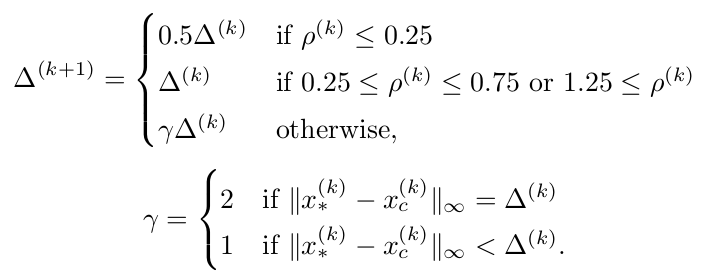
\includegraphics[width=0.55\textwidth]{images/TRMMcriteria.png}
\end{figure*}
The design optimization using trust regions begins with high- and low-fidelity function and gradient
evaluations at the initial design point. An initial trust region is formed using a prescribed initial size.
The approximate problem is formed, and optimized using an optimization
algorithm of choice. Once the sub-optimization has converged, the trust region is re-centered about the
approximate optimum, and the high-fidelity objective and gradient are evaluated. Convergence of the outer
loop optimization is checked. If the outer optimization has not converged, the ratio of actual versus predicted
improvement is determined and the trust region expanded or contracted accordingly. Using the data at the
new design point, an updated approximate problem is constructed, and the process is repeated until the
termination criteria are reached \cite{Bryson2019a}.
\subsection{Justification of the potential degree of novelty}
Most of the aforementioned research focuses on models that consider the inner disciplines of the MDO as black-box solvers. The outputs of both fidelities are parsed through statistical processes in order to create surrogate models that are then evaluated at each iteration of the optimizer. In many cases, the low fidelity model is actually a surrogate tailored to the behaviour of the high fidelity solver. On the other hand, the current strategy uses two indepedent ways to model the same phenomena. In addition, this approach aims to leverage the advantages of open-source tools at every level (MDO architecture, structural solver, fluid solvers, post-processing) so that the creation of a surrogate is not needed and the exchange of information between fidelities occurs seamlessly. Furthermore, the present work would introduce a multifidelity strategy to the existing aerostructures package developed by Mas-Colomer \cite{mascolomer:tel-02023612}, a python library developed specifically to set up aerospace problems within the OpenMDAO platform.     
\subsection{Aims and objectives}
From the early stages of the project, a series of objectives were defined for the current period, as follows: 
\begin{itemize}
    \item Complete review of the State of the Art: Literature review required to define strategies, methods, tools, etc.
    \item Single fidelity MDO implementation: Solution of the sample problem with both fidelity levels, which will later be used as bulding blocks for the multifidelity code.
    \item Define multifidelity model management: Propose a way to coordinate both fidelities, their interconection and the criteria that triggers a change from one level to the next. 
\end{itemize}
Although the original schedule did not mention it, an initial multifidelity would have been very welcome at the end of this period, however, it was not possible to have it ready before the submission date for this report and thus it is expected to be ready by mid-September. Future work is outlined in sec. \ref{sec:conclusions}.

\section{Investigation Methods}
\label{sec:invest_meth}
A series of tools will be used together in order to create a complete multifidelity optimization solver. First of all, the Multidisciplinary Design Analysis has to be established. The current work uses the OpenMDAO platform \cite{openmdao_2019}, an open source python library that allows the user to create, solve and optimize a wide variety of coupled problems. As a complement to this tool, the aerostructures package \cite{mascolomer:tel-02023612} assists the user in the creation of aerospace-related problems within the platform. Two different diagram formats of the MDA problem to be solved iteratively using a Gauss-Seidel method are shown in fig. \ref{fig:MDAdiagram}. \par The MDAO architecture is MultiDisciplinary Feasible or MDF, this means that the coupled problem is solved completely before the output is sent to the outer-loop optimizer. One of the advantages being that the optimization process can be interrupted before converging and the result at any point will satisfy consistency constraints (but not necessarily optimization constrains) \cite{gray2013standard}. There are many different MDAO architectures, in this case, the MDF was chosen because of the relatively simple problem (only 2 disciplines involved) and the ease of formulation. Another widely used architecture is Individual Discipline Feasible (IDF). It decouples the MDA, adding consistency constraints, and giving the optimizer control  of the coupling variables. This strategy generates a problem that is potentially much larger than MDF, depending on the number of coupling variables \cite{gray2013standard}. A wide study of different MDAO architectures is out of the scope of the current problem. \par
\begin{figure}
    \centering
    \begin{tabular}{cc}
     \subfloat[$N^2$]{ 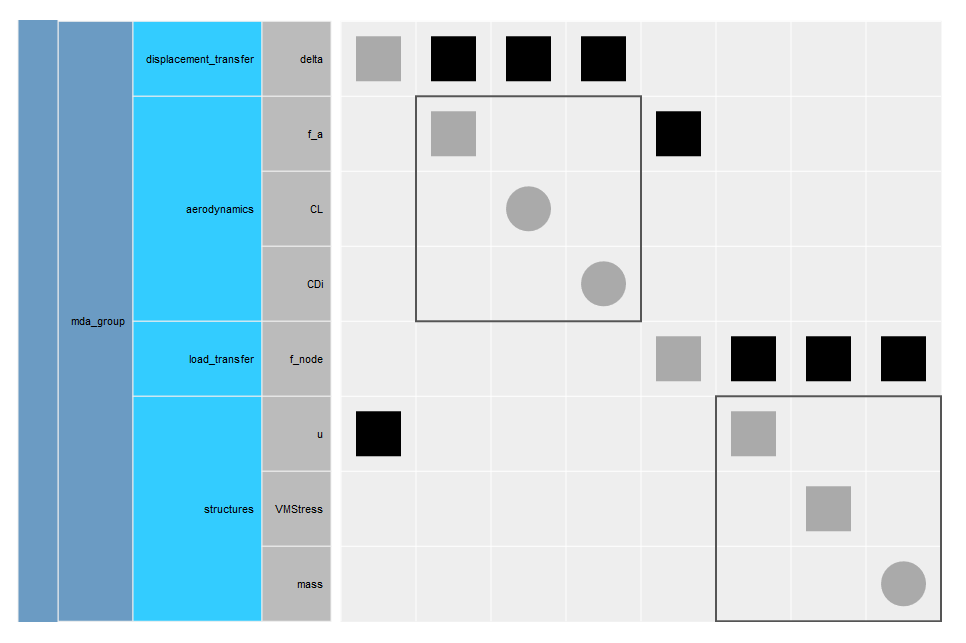
\includegraphics[width=0.45\textwidth]{images/MDAdiagram.PNG}}    & 
     \subfloat[XDSM]{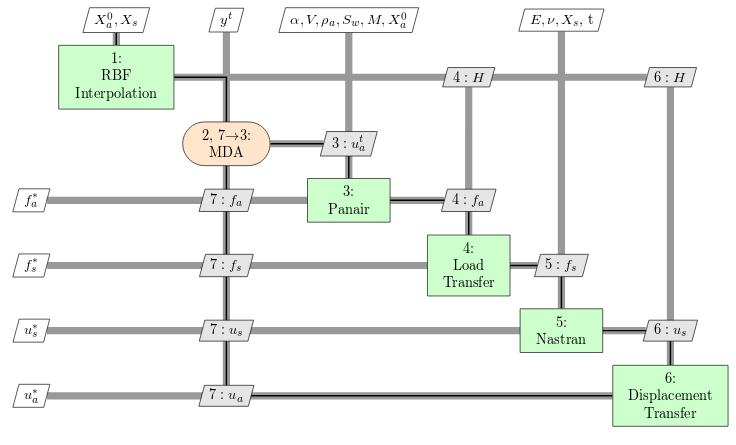
\includegraphics[width=0.5\textwidth]{images/XDSM.png}}
    \end{tabular}
    \caption{MDA diagrams of the coupled problem}
    \label{fig:MDAdiagram}
\end{figure}
High and low fidelity solvers were established to obtain the aerodynamic loads from the wing shape and the fluid characteristics. ADFlow is an open-source CFD code developed by the MDOLab at the University of Michigan. It solves the compressible Euler, laminar Navier-Stokes and Reynolds-Averaged Navier-Stokes equations \cite{lyu2013automatic}. On the other hand, PANAIR \cite{carmichael1981pan} was chosen as the low fidelity model. It is an open-source implementation of the potential flow theory via panel methods. Finally, post-processing of the data is achieved through python scripts that transform outputs from NASTRAN and PANAIR to mesh files (.msh) that can be opened in the open source software Gmsh \cite{geuzaine2009gmsh}. 

\section{Results and analysis}
\label{sec:results}
For simplicity reasons, a basic structure was used to test and develop the code before its final implementation on the BWB concept. The wing section of the NASA's Common Research Model \cite{vassberg2008development} was chosen as the starting geometry to be optimized. The objective function of the problem is the induced drag, $C_{d_i}$, with respect to a series of design variables, and respecting two main constraints: cruise lift and maximum Von Mises stress. These parameters are detailed in appendix \ref{sec:sampleprob}. The sample problem was set up using the low-fidelity solver and NASTRAN. Some slight changes were made on the original scripts to ensure compatibility with newer versions of Python. However, the overall strategy did not change. \par 
The optimized solution showing Von Mises stress is shown in fig. \ref{fig:lowfi_res}a, the $C_p$ distribution was computed as well (see fig. \ref{fig:lowfi_res}b). Both results are presented over the optimized geometry. Aside from the equivalent stress and $C_p$ distribution, it is interesting to look at the objective function convergence and the constraint evaluation plots. These are displayed in fig. \ref{fig:solcontr}, please note that they correspond to the outer loop of the MDAO problem, not the MDA that must be solved iteratively for every step of the optimizer. A single example of the coupled probem solution is shown in fig. \ref{fig:solmda}, it is at this level that an alternation between fidelities is proposed.  It takes 286 iterations of the optimizer for the model to converge in low fidelity mode to a $C_{d_i}$ of 0.00718. \par 
Once the multifidelity model is ready, a performance comparison will be carried out between both methods. The main parameters for the comparison will be the total execution time and the distance to the optimum and to the normalized constraints. An equivalent implementation of the problem using a High-Fidelity solver was also reviewed as a way to get familiar with its functioning. The computing time in this case is significantly larger compared to the previous one, some issues with the server were ADFlow is located prevented the implementation of this code.  

\begin{figure}
\centering
\begin{tabular}{c}
\subfloat[Von Mises stress, aerodynamic mesh shown for reference. (Pa)]{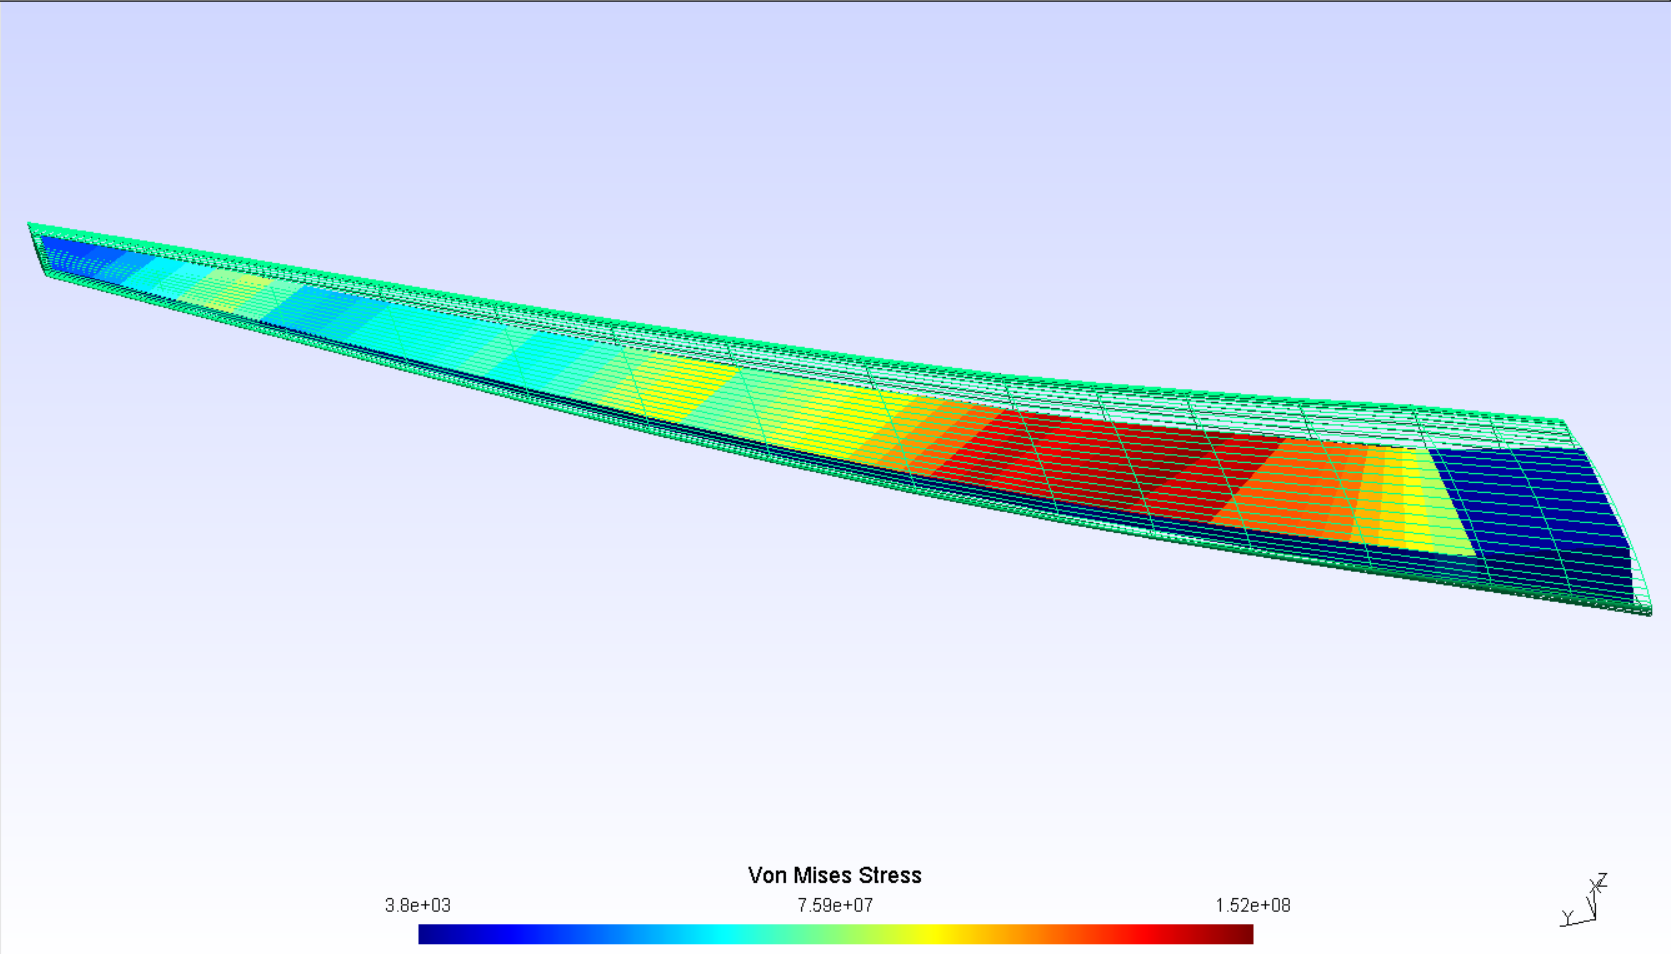
\includegraphics[width = 0.75\textwidth]{images/structure_aeromesh.png}} \\
\subfloat[$C_p$ distribution]{\includegraphics[width = 0.75\textwidth]{images/cplowfi.png}} 
\end{tabular}
\caption{Optimized wing section for the low-fidelity implementation.}
\label{fig:lowfi_res}
\end{figure}

\begin{figure}
\centering
\begin{tabular}{ccc}
\subfloat[]{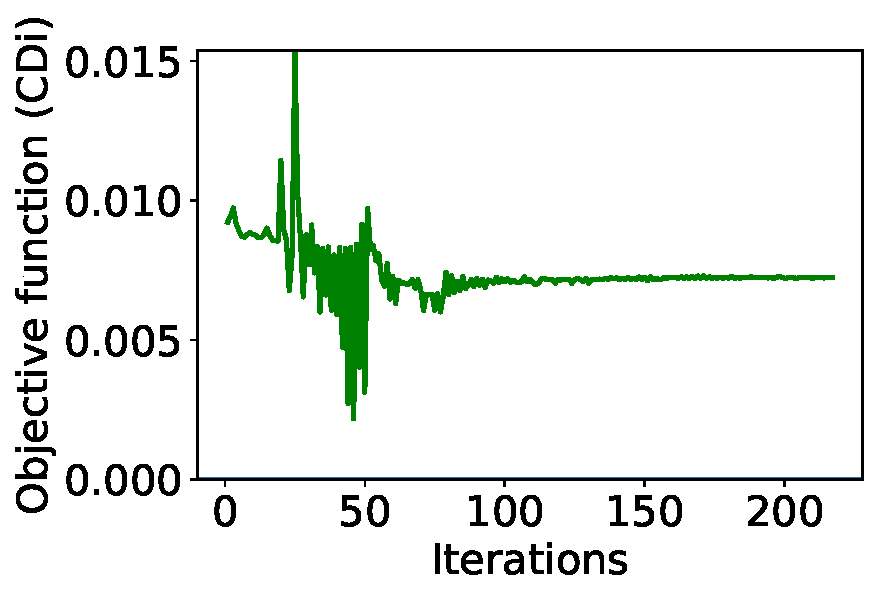
\includegraphics[width = 0.30\textwidth]{images/objective_cdi.pdf}} &
\subfloat[]{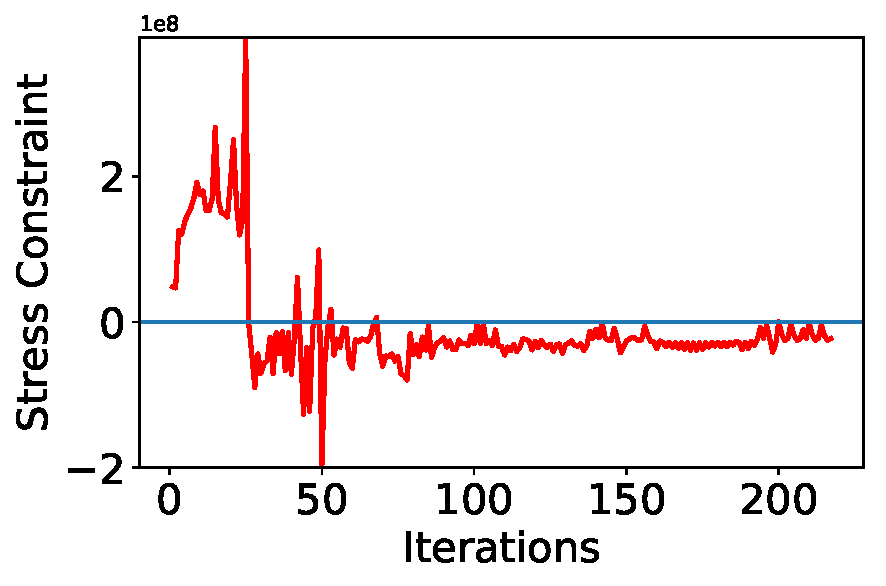
\includegraphics[width = 0.30\textwidth]{images/stress_constraint.pdf}} &
\subfloat[]{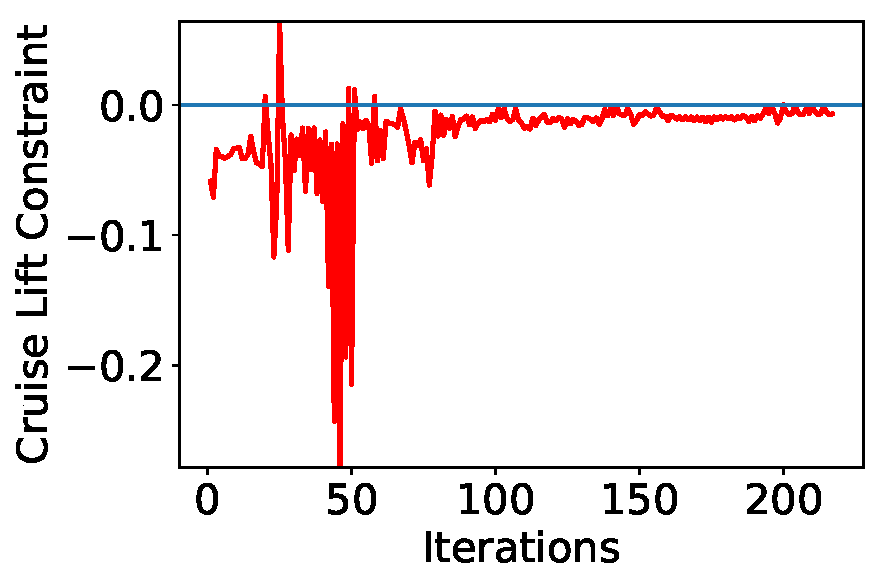
\includegraphics[width = 0.30\textwidth]{images/cruise_lift_constraint.pdf}} 
\end{tabular}
\caption{Objective function, stress constraint and cruise lift constraint plots.}
\label{fig:solcontr}
\end{figure}

\begin{figure}
\centering
\begin{tabular}{cc}
\subfloat[]{\includesvg[width=0.4\textwidth]{images/plot_unknowns_norm}} &
\subfloat[]{\includesvg[width=0.4\textwidth]{images/plot_wingtip_disp}} 
\end{tabular}
\caption{Solution convergence for one sample step of the MDA}
\label{fig:solmda}
\end{figure}

\section{Conclusions and perspectives}
\label{sec:conclusions}
Up to this point, the main tasks of the present work were the state of the art review and the implementation of sample problems in Single-Fidelity mode in order to get acquainted with the various tools required to create the multifidelity optimization. 
Future work for S3 includes writing the python code that connects both fidelity levels within the OpenMDAO environment. This will allow the optimization of the sample case, which in turn can be used as a bench-marking reference to review the performance of the new proposal versus single-fidelity implementations. Depending on the results, minor or major changes will be applied to the multifidelity code in order to improve its efficiency. Once the method handles properly the sample case, a BWB configuration will be optimized and the results will be validated using academic sources. Since the complexity of the problem will increase, a second performance review of the code will be carried out to check for any possible improvements.   
